\documentclass[12pt,aspectratio=169]{beamer}
\usetheme{iiasa}

\usepackage{ifthen}
\ifthenelse{\equal{\detokenize{notes}}{\jobname}}{%
\setbeameroption{show only notes}%
}{
%
}

\usepackage[
  maxnames = 1,
  style = authoryear,
  giveninits,
  terseinits,
  maxcitenames = 3,
  ]{biblatex}
\addbibresource{all.bib}

% \usepackage{minted}
\usepackage[normalem]{ulem}

\title{Modeling low carbon transport development}
\subtitle{Considerations for selecting, building, and using models}
\institute{Energy, Climate, and Environment (ECE) Program \\
  International Institute for Applied Systems Analysis (IIASA)}

\date{\scriptsize
  \texorpdfstring{UN ESCAP Regional Cooperation Mechanism on Low Carbon Transport: Establishment and Implementation of Low Carbon Transport Targets and Timelines in Asia and the Pacific\\
  \structure{Wednesday, 17 July 2024}}%
  {2024-07-17}}

\author{\texorpdfstring{Paul Natsuo Kishimoto\scriptsize\newline
  \href{mailto:paul.kishimoto@iiasa.ac.at}%
       {\ttfamily <paul.kishimoto@iiasa.ac.at>}}%
  {Paul Natsuo Kishimoto <paul.kishimoto@iiasa.ac.at>}}

\begin{document}

\maketitle

\begin{frame}
\frametitle{Introduction}
\structure{Not} a sales pitch for our particular model, “MESSAGEix-Transport”…

\onslide<2>{
\begin{itemize}
  \item \url{https://docs.messageix.org/models} —specific model \& general framework.
  \item \textcite{mccollum-2017} —prior version.
\end{itemize}}

\bigskip
…instead:
\smallskip
\begin{quote}
    \large
    How should you—policymakers, or researchers providing policy guidance—\structure{select, build, and use} models and other tools within model-based assessments of low-carbon transport development?
\end{quote}

\end{frame}

\begin{frame}
\frametitle{Outline}
\tableofcontents
\end{frame}

\section{General considerations}

\subsection{Credible, salient, legitimate}
\begin{frame}
\frametitle[allowframebreaks]{Credible, salient, legitimate}
\framesubtitle{\cite{cash-2003}}

Models are not the start, end, or goal \emph{per se}.

\bigskip
They are one piece in iterative, multi-stakeholder \structure{processes of policy option assessment} where they are \structure{tools for analysis} and \structure{knowledge objects}.

\bigskip
Processes are successful if they are:

\begin{description}
  \item [Credible] carried out with scientific validity in methods and data.
  \item [Salient] produce results that are relevant to the policy decisions or questions.
  \item [Legitimate] involve stakeholders (institutions, individuals) or show that their concerns are heard and represented.
\end{description}

\end{frame}

\subsection{Costs \& resources}
\begin{frame}
\frametitle{Costs \& resources}
\framesubtitle{Time/money for tasks associated with model-based assessment}

\begin{columns}[T]
\column{0.6\textwidth}
\begin{itemize}
  \item Understand methods and capabilities of different model frameworks.
  \item Hire and train staff capable to construct \& operate model.
  \item Collect and prepare input data.
  \item Design scenario narratives and quantifications.
  \item Extend model methods.
  \item Interpret and present output data and results.
  \item Iterate.
\end{itemize}

\column{0.4\textwidth}
Any tool (or set of tools) offers certain \structure{affordances}: it can make each of these tasks \structure{easier} (less costly) or \structure{harder}.

\bigskip
→ There is no ‘right’ or ‘best’ model; only those that can be used with available resources to produce C/S/L results.
\end{columns}

\end{frame}

\section{What to ask}

\begin{frame}
\frametitle{“What to ask”}

The only responsible way for policymakers/stakeholders to use limited resources is to choose model frameworks, build models, prepare data, etc. that \structure{are capable to support C/S/L policy assessment}.

\bigskip
Therefore, they must ask: \structure{Can we do C/S/L/ assessment using this model framework?}

\bigskip
Researchers, analysts, and others proposing the use of particular model frameworks and tools must be able to \structure{answer this question}.
If answers are not offered or satisfactory, the tool is probably not the right choice.

\end{frame}

\subsection{Complexity}
\begin{frame}
\frametitle{Complexity of systems vs. models}
\framesubtitle{\href{https://mitpress.mit.edu/books/engineering-systems}{de Weck, Roos, Magee (2011) fig. 3.1, p.47}}

\begin{columns}
\column{0.6\textwidth}
\includegraphics[height=0.78\textheight]{de-weck-roos-magee-f3.1}

\column{0.4\textwidth}
Real-world transport systems are unavoidably \structure{complex}.

\medskip
Models \emph{should} be \structure{parsimonious}: use the simplest possible methods \& least possible data that explain the largest part of the output.
But:

\begin{itemize}
  \item Model-builders enjoy (or are motivated) to make models \structure{complicated}.
  \item Making parsimonious methods is costly.
\end{itemize}
\end{columns}

\end{frame}

\begin{frame}
\frametitle{Complexity of systems vs. models}
\framesubtitle{What to ask}

\begin{itemize}
  \item Is the model framework \structure{explainable}?
    How hard is it to understand and communicate \emph{why} it gives certain results?
  \item Is the model framework \structure{complicated to use}?
    Has the pursuit of detail made it costly to set up and run a model, and analyse the results?
  \item Does the model framework include \structure{irrelevant} (=not salient) details?
    If there are options to turn off certain features, reduce resolution, etc., this can reduce the cost of using the model.
\end{itemize}

\end{frame}

\subsection{Scope, resolution}
\begin{frame}
\frametitle{Scope and resolution}
All model data & methods have \structure{conceptual dimensions}—especially \uline{space} and \uline{time}, but often many others like \uline{transport service}, \uline{transport mode}, \uline{trip purpose}, \uline{vehicle type}, \uline{fuel type}/energy carrier, etc.

\bigskip
For every model framework, \structure{ask}:
\begin{itemize}
  \item What conceptual dimensions are included \emph{explicitly}?
  \item What approach (averaging, aggregation, scenarios) are taken for \emph{other} dimensions that are \emph{not} explicit?
\end{itemize}

\bigskip
For every dimension, \structure{ask} about two characteristics:
\begin{description}
  \item [Scope] What is included/excluded along this dimension?
    e.g. “national model” may mean “spatial scope = 1 country”.
  \item [Resolution] How many different categories, units, etc. are represented?
    e.g. “national model” may mean “spatial resolution = entire countries”
\end{description}

\end{frame}

\begin{frame}
\frametitle{Scope and resolution: examples}

\begin{columns}
\column{0.55\textwidth}[T]
“National model”
\begin{itemize}
  \item …could mean spatial \uline{scope} = 1 country.
  \item …could mean spatial \uline{resolution} = entire countries (e.g. total passenger activity for all people); scope unclear.
\end{itemize}

\bigskip
“Model of electrification”
\begin{itemize}
  \item Refers to the “fuel type” concept.
  \item Could mean \uline{scope} = electricity only.
  \item Could mean \uline{resolution} = \{electricity, other\}
\end{itemize}

\column{0.45\textwidth}
Also relates to \structure{model purpose}: e.g. global integrated assessment models (IAMs) are made to study global, economy-wide climate policy.
\begin{description}
  \item [Spatial] \uline{scope} must be global → \uline{resolution} is very coarse; ~10 groups of countries.
  \item [Temporal] \uline{scope} must be long-term (2100+) → \uline{resolution} may be coarse; 5–10 year periods.
\end{description}
\end{columns}

\end{frame}

\subsection{Phenomena represented}
\begin{frame}
\frametitle{Phenomena represented}

\begin{columns}[T]
\column{0.5\textwidth}
\structure{Phenomena} include existing dynamics or change that happens in, or to, transport systems.
\begin{itemize}
  \item Population \& income growth.
  \item Policy to encourage telecommuting.
  \item Change of costs (subsidy, tax) of activity or technologies.
  \item Information provision.
\end{itemize}

\medskip
Every phenomenon has a \structure{natural unit of analysis} where it is best measured and modeled.

\column{0.5\textwidth}
Models may \structure{“capture”} these in different ways:
\begin{description}
  \item [Directly] if scope and resolution allow.
  \item [Aggregate] by changing totals or other values at lower/coarser resolution than the natural unit of analysis.
  \item [Scenarios] of alternate possibilities.
  \item [...] others.
\end{description}

\end{columns}

\end{frame}

\begin{frame}
\frametitle{Phenomena represented}
\framesubtitle{What to ask}

\begin{itemize}
  \item Which \structure{categories of phenomena} and \structure{specific phenomena} are explicitly represented in the model?
  \item For others not represented, what approach is taken?
  \item Which are not included at all?
\end{itemize}

\bigskip
Important to recall that “the map is not the territory”: no model (framework) will include everything that happens in the real world.

\end{frame}


\subsection{Data availability}
\begin{frame}
\frametitle{Data availability}
\framesubtitle{Cost (time, money) obtain necessary inputs (1)}
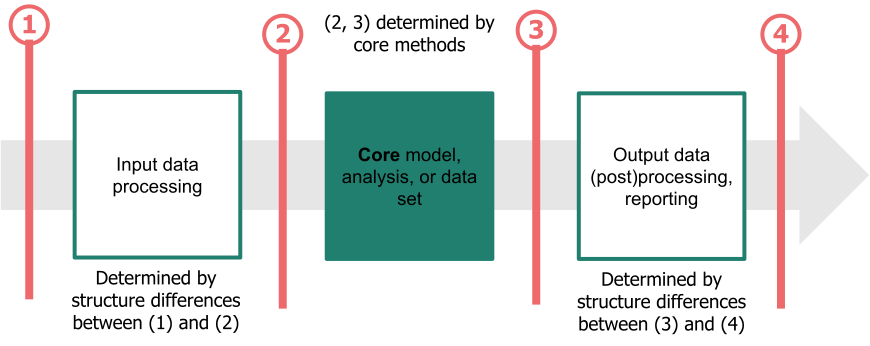
\includegraphics[width=\columnwidth]{data-stages}
\end{frame}

\begin{frame}
\frametitle{Data availability}
\framesubtitle{What to ask}
\begin{itemize}
  \item What are the \structure{minimum data requirements} of the model/method?
    \begin{itemize}
      \item Which quantities/measures?
      \item For each one, what are its dimensions, and scope and resolution along those dimensions?
    \end{itemize}
  \item Does the model framework come with \structure{tools to obtain/prepare data}?
  \item If the data is \structure{not available}, can they be easily filled with \structure{placeholders or assumptions}?
    \begin{itemize}
      \item Are there references, literatures, or proxy data available on which to make these assumptions?
      \item Are there existing examples?
    \end{itemize}
  \item Do these data needs align with \structure{available data} in my country \& context?
\end{itemize}

\end{frame}

\subsection{Free \& open source}
\begin{frame}
\frametitle{Free \& open source}

Select model frameworks that are \structure{free \& open source}.

\begin{description}
  \item [Transparency → validity] Many eyes looking at the code that implements methods can help ensure it is correct.
  \item [Support \& community] Shared tools attract a community of users who can offer help with common technical hurdles.
  \item [Quality assurance] Model software that is published and actively maintained will have bug fixes and support available.
\end{description}

\bigskip
Make your concrete models free and open source.
\begin{itemize}
  \item Best way to build legitimacy and fix issues for better credibility.
  \item Motivated researchers and others will offer contributions.
  \item Consultants and advisors can dive directly into methods and check/offer advice.
\end{itemize}

\end{frame}

\begin{frame}
\frametitle{Concluding thoughts}

It is good and healthy to “let a hundred flowers blossom”:
\begin{itemize}
  \item There are many types of policy assessments, and each has different modeling needs.
  \item Scientific research requires \emph{experimentation} with alternate methods to determine which are useful for which purposes.
\end{itemize}

\bigskip
However, given the imperative of sustainable human development and climate change mitigation \& adaptation, we must make clear, principled, and \structure{context-appropriate choices} of tools and methods.
\end{frame}

\begin{frame}[plain]
  \centering \Huge \structure{Thank you!}
\end{frame}

\appendix

\section{References}

\begin{frame}
\frametitle{References}

\printbibliography[heading=none]

\end{frame}

\end{document}
